
\chapter{The item/system problem}
\label{itemsystemproblem}
\is{item/system problem}


When accounts of social-cultural transmission are explicit about the 
causal processes involved, they often take cultural \textit{items} -- rather than systems -- as their unit of analysis. This works well 
but it is awkward because we know that cultural items don't exist in 
isolation. We can only make sense of cultural items in the context of a 
\textit{system} of cultural meaning.\is{systems} This brings us back to the puzzle, foreshadowed in Chapter \ref{causalunits}, of causal units. 



Higher-level systems like languages and cultures show enormous coherence 
of structure, so much so that we are seduced into thinking of them as organisms with 
bodies (see classic statements of philologists \citealt{gabelentz_sprachwissenschaft_1891} and \citealt[16]{meillet_linguistique_1926}). Here is Gabelentz:

\begin{quotation}
Language is not a mere collection of words and forms, just as the organic body is not a mere collection of limbs and organs. Both are in any stage of their life (relatively) complete systems, dependent on themselves; all their parts are interdependent and each of their vital manifestations arises from this interaction. \citep[10]{gabelentz_sprachwissenschaft_1891}
\end{quotation}

Compare this to the situation in vertebrate\is{vertebrates} 
biology. Genes\is{genetics} are distinct entities yet they ``form 
alliances'' thanks to the bodies and body plans in which they are 
instantiated (\citealt{gould_ontogeny_1977}, cited in \citealt[117]{dawkins_extended_1982}). 

\begin{quotation}
Every gene in a gene pool constitutes part of the environmental background against which the other genes are naturally selected, so it's no wonder that natural selection favors genes that `cooperate' in building these highly integrated and unified machines called organisms.  Biologists are sharply divided between those for whom this logic is as clear as daylight, and those (even some very distinguished ones) who just do not understand it -- who naively trot out the obvious cooperativeness of genes and unitariness of organisms as though they somehow counted against the `selfish gene' view of evolution. ... By analogy with coadapted gene complexes, memes, selected against the background of each other, `cooperate' in mutually supportive memeplexes. \citep[xv]{DawkinsMemeForeword1999}
\end{quotation}

Vertebrates have bodies while cultural systems 
do not. Still, the item/system link needs to be accounted for in both cases. With both bodies and memeplexes,\is{memes} sets of items somehow hold together as systems. But the causal forces are different. The pieces of a cultural system are not held together at any stage by physical 
attachment to a shared material whole. So this is our puzzle. If 
languages and other cultural systems hang together, what is the 
binding force? We have seen that cultural transmission involves causal processes that 
apply only to small parts of the larger whole. What explains the 
coherence of that larger whole? This is the item/system problem.



Here is the solution. The ideas of cultural item and cultural system are reconciled by something that they have in 
common: Neither idea exists without the simpler idea of a \textit{functional relation}.\is{functional relation} A word -- \textit{kangaroo}, for example -- is easily thought of as a 
distinct cultural item. You can cite it or borrow it without having to 
also cite or borrow the language system that it comes from. But the word 
cannot be defined or understood -- nor can it exist -- except in terms of its 
functional relation to other things, things like the words it co-occurs 
with, the conversations in which it is used for referring to kangaroos, 
and so on. The same is true for technology. A spoke\is{spoke and wheel} can be designed, named, bought, and sold, 
but as a cultural item, a spoke doesn't make sense without a wheel. And 
while a wheel is a whole when thought of with reference to a spoke, it 
is a \textit{part} when thought of with reference to a vehicle, and so 
on. 



In sum: An item doesn't make sense without functional relations to other 
things, just as a system doesn't make sense without the functional 
relations that it contains. Functional relations are the interface that 
joins items and systems together. We can look to functional relations for a solution 
to the item/system problem.

\section{A transmission criterion}

\is{transmission criterion}
In the causal ontology of culture, there is a \textit{transmission 
criterion}. A social fact -- by definition -- would cease to exist if 
individual people stopped behaving as if it existed \citep{searle_making_2010}. And social facts 
endure with relative stability beyond individual people's lifetimes. Therefore, social facts must be transmitted among individuals in human 
populations in order to (i) exist and (ii) endure with relative 
stability. Transmission is a necessary part of what makes culture and 
language the way they are. 



A causal understanding of culture depends, then, on knowing how culture is transmitted within human groups and across 
generations. Much is known about how \textit{items} are transmitted 
\citep{rogers_diffusion_2003}, but macro-level cultural systems cannot be 
transmitted in the same way. 



Do we need two separate accounts of transmission, one for items, one for 
systems? I am going to argue that we can derive system transmission from 
item transmission, on the condition that we have a more accurate 
definition of \textit{items}. We can define items not as cultural things but as 
cultural things with functional relations to other cultural things. 
Cultural items are specified for -- and advertize -- their relations to the 
contexts into which they fit (where, it must be said, this fit can be 
quickly and easily re-tooled). As \citet[19]{kockelman_agent_2013} writes: ``there 
are no isolated environments and organisms, there are only \textit{envorganisms}.''\is{envorganism} 

\section{Defining properties of systems}

\is{systems}
To understand what a cultural system is, begin with the idea of a cultural item.\is{linguistic item} This is any seemingly detachable conceived entity such 
as a piece of technology, a technique, a way of saying something, a 
value. An item can be readily defined and labeled, and can be learned 
and borrowed from one human group into another (though typically with 
a change of meaning in the new context). Object-like 
things such as tomahawks might be prototypical items, but the idea of 
item intended here also includes train tracks, AC current, and 
mother-in-law avoidance. 



By contrast, a cultural system is a coherent \textit{set} of such items, each 
item related to the others. A system has a holism that goes 
beyond the sum of the parts, in the sense that the full meaning of any 
individual cultural item is determined by how it functions in relation to other things in context. Often, we cannot observe the system directly or in one go, as for 
example in the case of a language or a telecommunications 
infrastructure, though this is sometimes made virtually possible by 
means of \textit{signs of} these systems that scale them down in such 
a way as to produce a ``tangible expression'', as \citet[208]{durkheim_elementary_1912} put it, of the more diffuse phenomenon. 



A book can contain a grammatical description of a language. A diagram 
can portray the elements of a telecommunications system in miniature. In 
these cases a representation of the system is created or inferred 
from an aggregate of encounters with context-situated items. These 
itemized emblems are different from the real systems they 
represent, and they have different collateral effects as a result of 
their form. A grammar book,\is{grammars} for example, can be held up in one hand. This helps to promote the idea that a 
language is a finite, bounded thing; in short, an item. 



As we now turn to examine systems in more detail let me emphasize that neither items nor systems can be understood, nor indeed can 
they exist, without the \textit{relations }that are inherent in both. 
Relations are definitive for both items and systems. If something is an item, 
relations define its \textit{functions}. If it is a system, relations 
define its \textit{structure}.



A system should have at least these three properties:\is{systems} 


\begin{enumerate}
\item It can readily be construed as a thing with multiple inter-related parts.

\item Effects on one part should have effects on other parts.

\item The parts should together form a whole in the sense that they are more closely related to each other than they are to things outside the system. 

\end{enumerate}


Good examples are biological or ecological systems. In a food chain,\is{food chain, as system} 
populations of different species are inter-related. Changes in the 
frequency or behavior of one species will affect the frequency or 
behavior of others. While each species in the ecosystem will ultimately 
be connected to entities outside the focal food chain system, the 
integration \textit{within }the system is greater. 



Clearly, on all three counts, whether or not we are looking at a system 
is ultimately a matter of construal. %(see fn. 10, above).  
To say that some entities form a system is partly just a way of looking at those 
entities. 


%\textit{note:} \textquoteleft There is evidence that grammatical change is not always limited to the language acquisition process. The grammar of an adult can change.' (H\&C:49)
%'[T]he grammar of an adult is best viewed, not as an inflexible completed object, but as an adaptable, constantly growing set of generalisations.' (H\&C:49)


\section{Relations between relations}
\is{relations between relations}

Culture and language hinge on shared meaning, and so the systems we are interested in here are \textit{semiotic }systems. The core idea of a semiotic system 
is well illustrated in Darwin's account of the expression of emotion\is{emotion} in 
animals. Darwin introduces a principle of \textit{functional connection 
}between a sign and what it stands for. 



In his example, the visible features of a dog in a ``hostile frame of 
mind'' -- upright, stiff posture, head forward, tail erect and rigid, 
bristling hairs, ears forward, fixed stare -- are intelligible because they 
recognizably ``follow from the dog's intention to attack''. \figref{darwin1} is 
Darwin's illustration.


\begin{figure}[p]
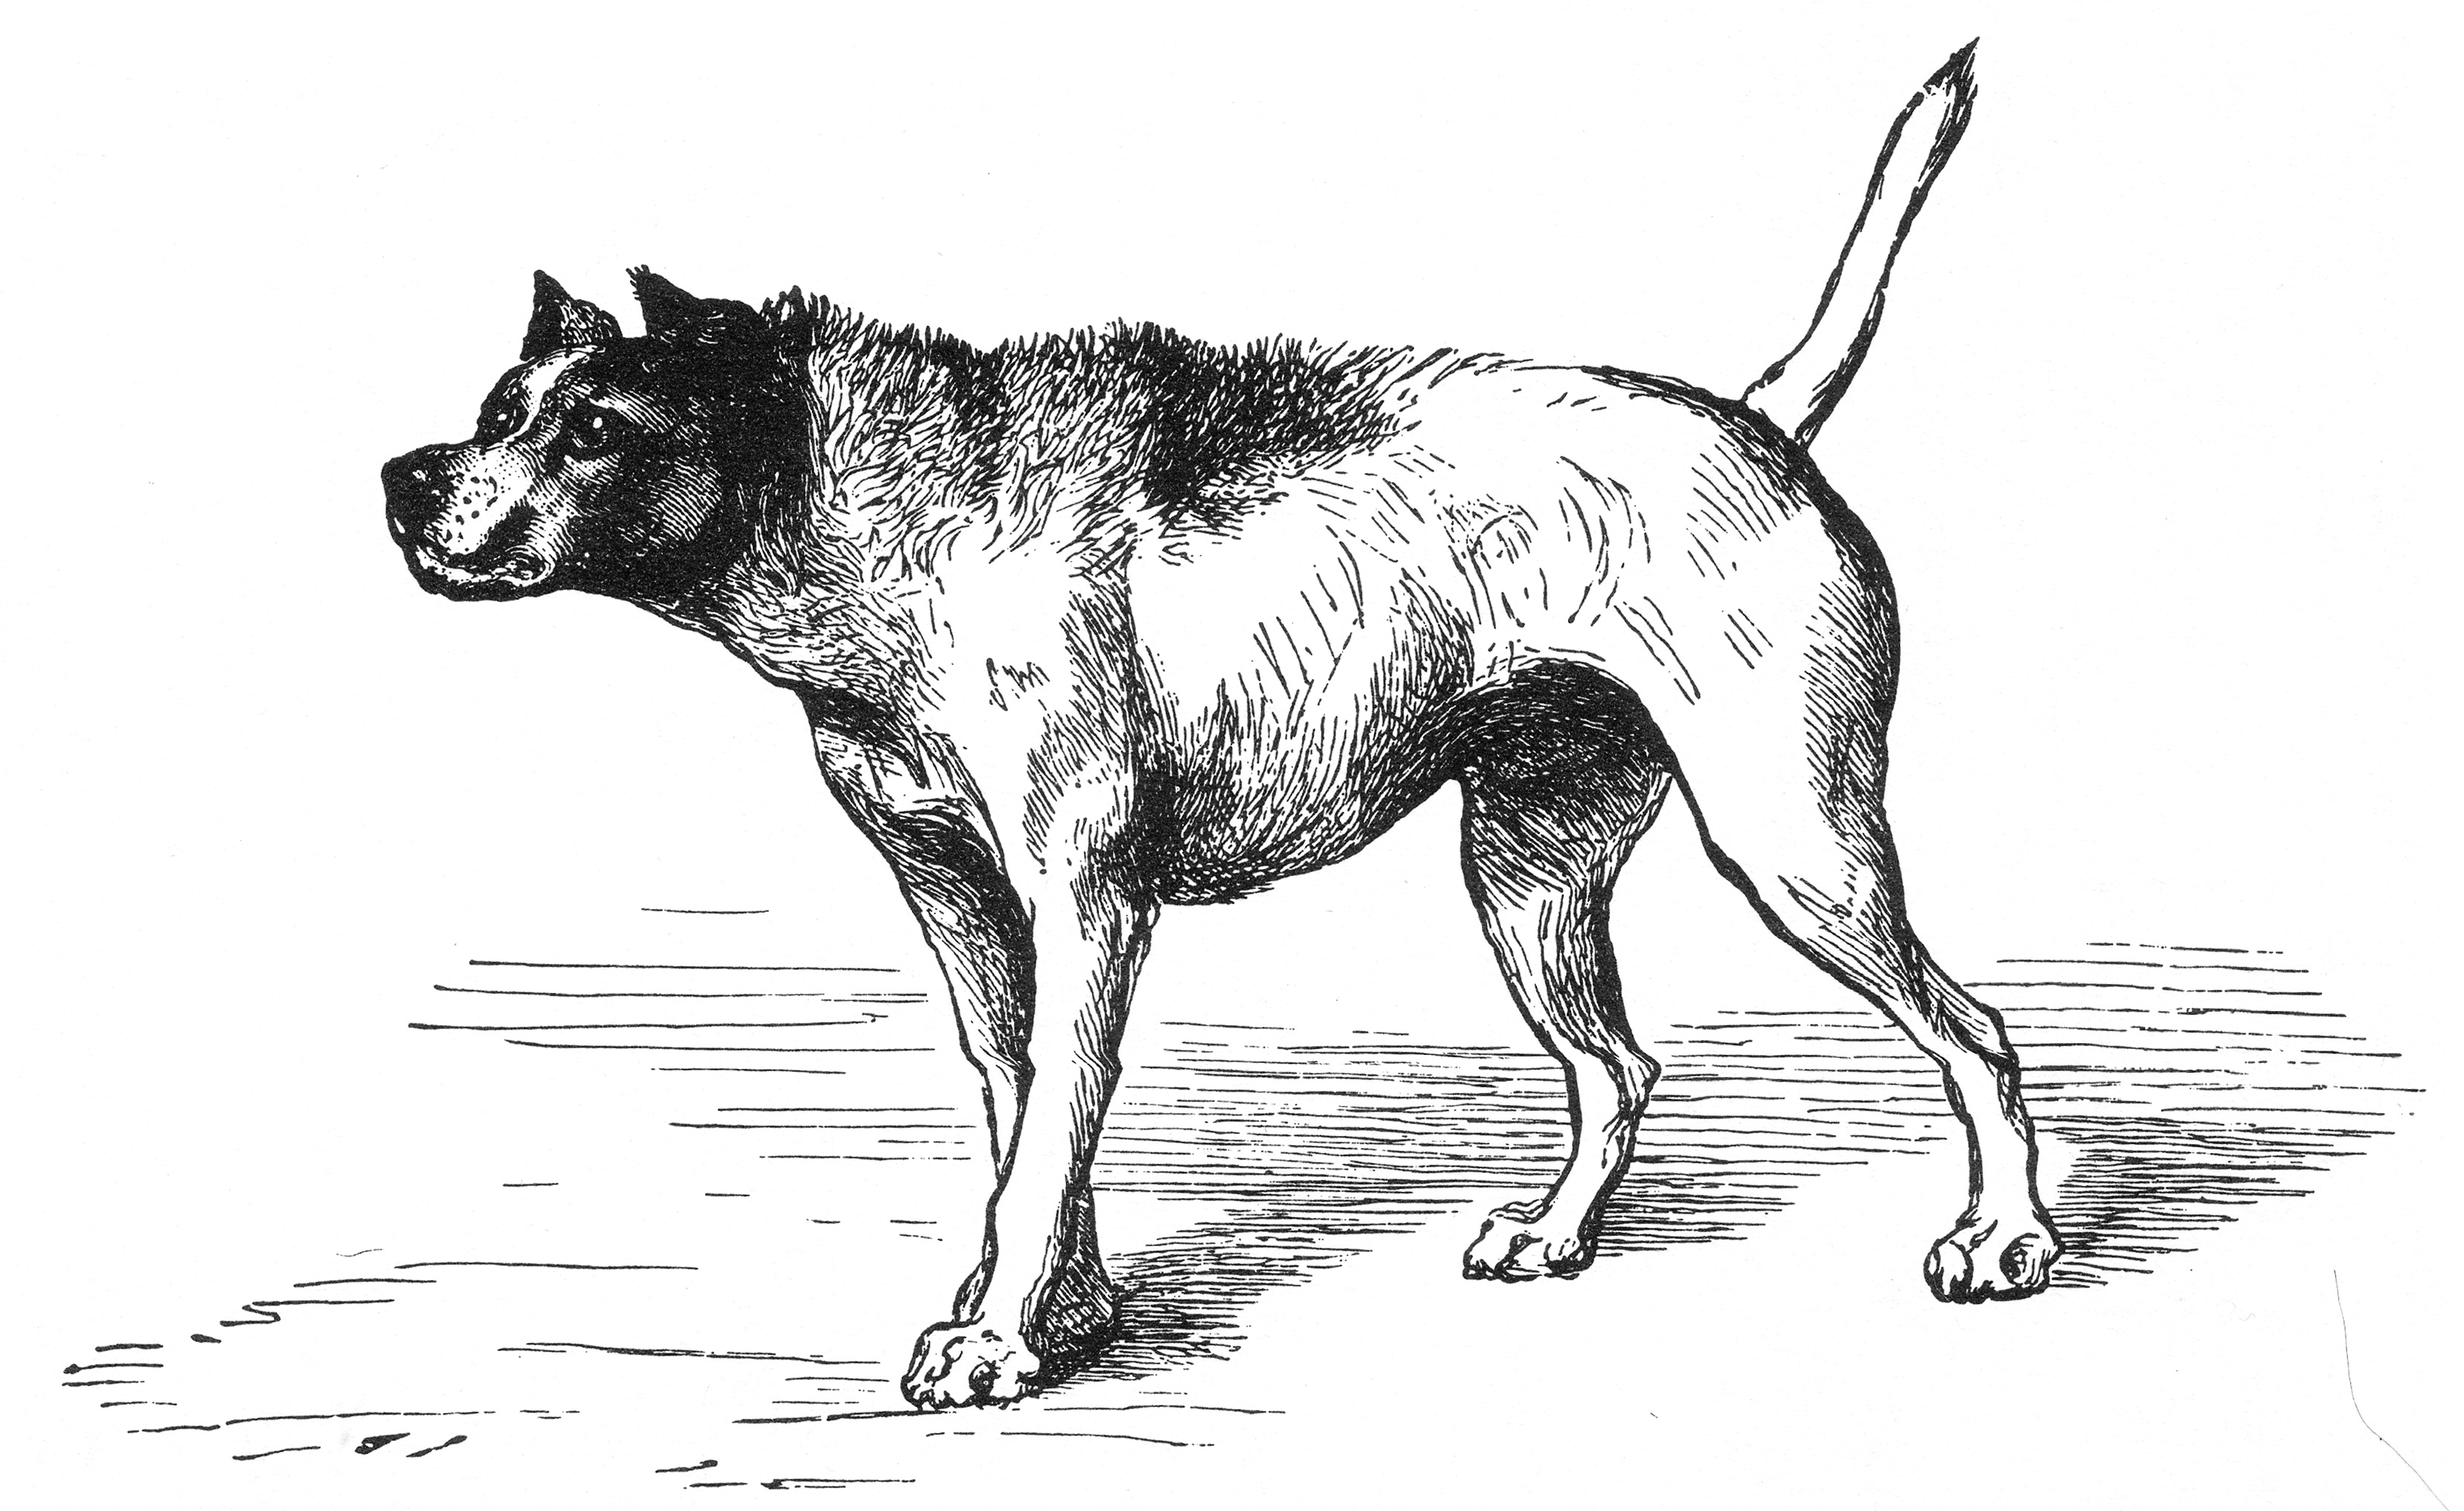
\includegraphics[width=0.70\textwidth,keepaspectratio]{figures/Fig01}
\caption{Darwin's illustration of a dog in hostile frame of mind 
(Figure 5 from \textit{The Expression of the Emotions in Man and 
Animals}).}
\label{darwin1}
\end{figure}



These behaviors are functionally connected to the aggressive attitude, 
and so others may take them to signal that attitude. This can be illustrated as in  \figref{functionalassoc}.

\begin{figure}[p]
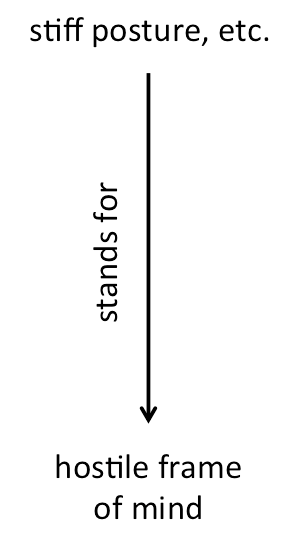
\includegraphics[width=0.22\textwidth,height=\textheight,keepaspectratio]{figures/Fig02}
\caption{A ``functional'', indexical association between observable 
behavior and frame of mind (after Darwin).}
\label{functionalassoc}
\end{figure}


This is only a first step toward establishing a semiotic system. Figure 
\ref{functionalassoc} shows a relatively simple semiotic relation. There is a potential positive association\is{functional association} between an 
observable behavior and a frame of mind. Whoever makes this association might produce a 
number of relevant interpretants, for example running away, grabbing a big 
stick, or adopting an attacking posture. 



Darwin then argues for a second signalling principle, which he calls \textit{antithesis}.\is{antithesis} The dog can exploit the already established semiotic 
relation shown in \figref{functionalassoc} to express the \textit{opposite} 
of aggression. He does this by ``reversing his whole bearing'', that is, doing the 
`opposite'\is{opposite} of what he would do when aggressive. So, when approaching 
his master in an affectionate attitude, his visible behaviors will include body 
down, flexuous movements, head up, lowered wagging tail, smooth hair, 
ears loosely back, loose hanging lips, eyes relaxed. \figref{darwin2} is 
Darwin's illustration.


\begin{figure}[h]
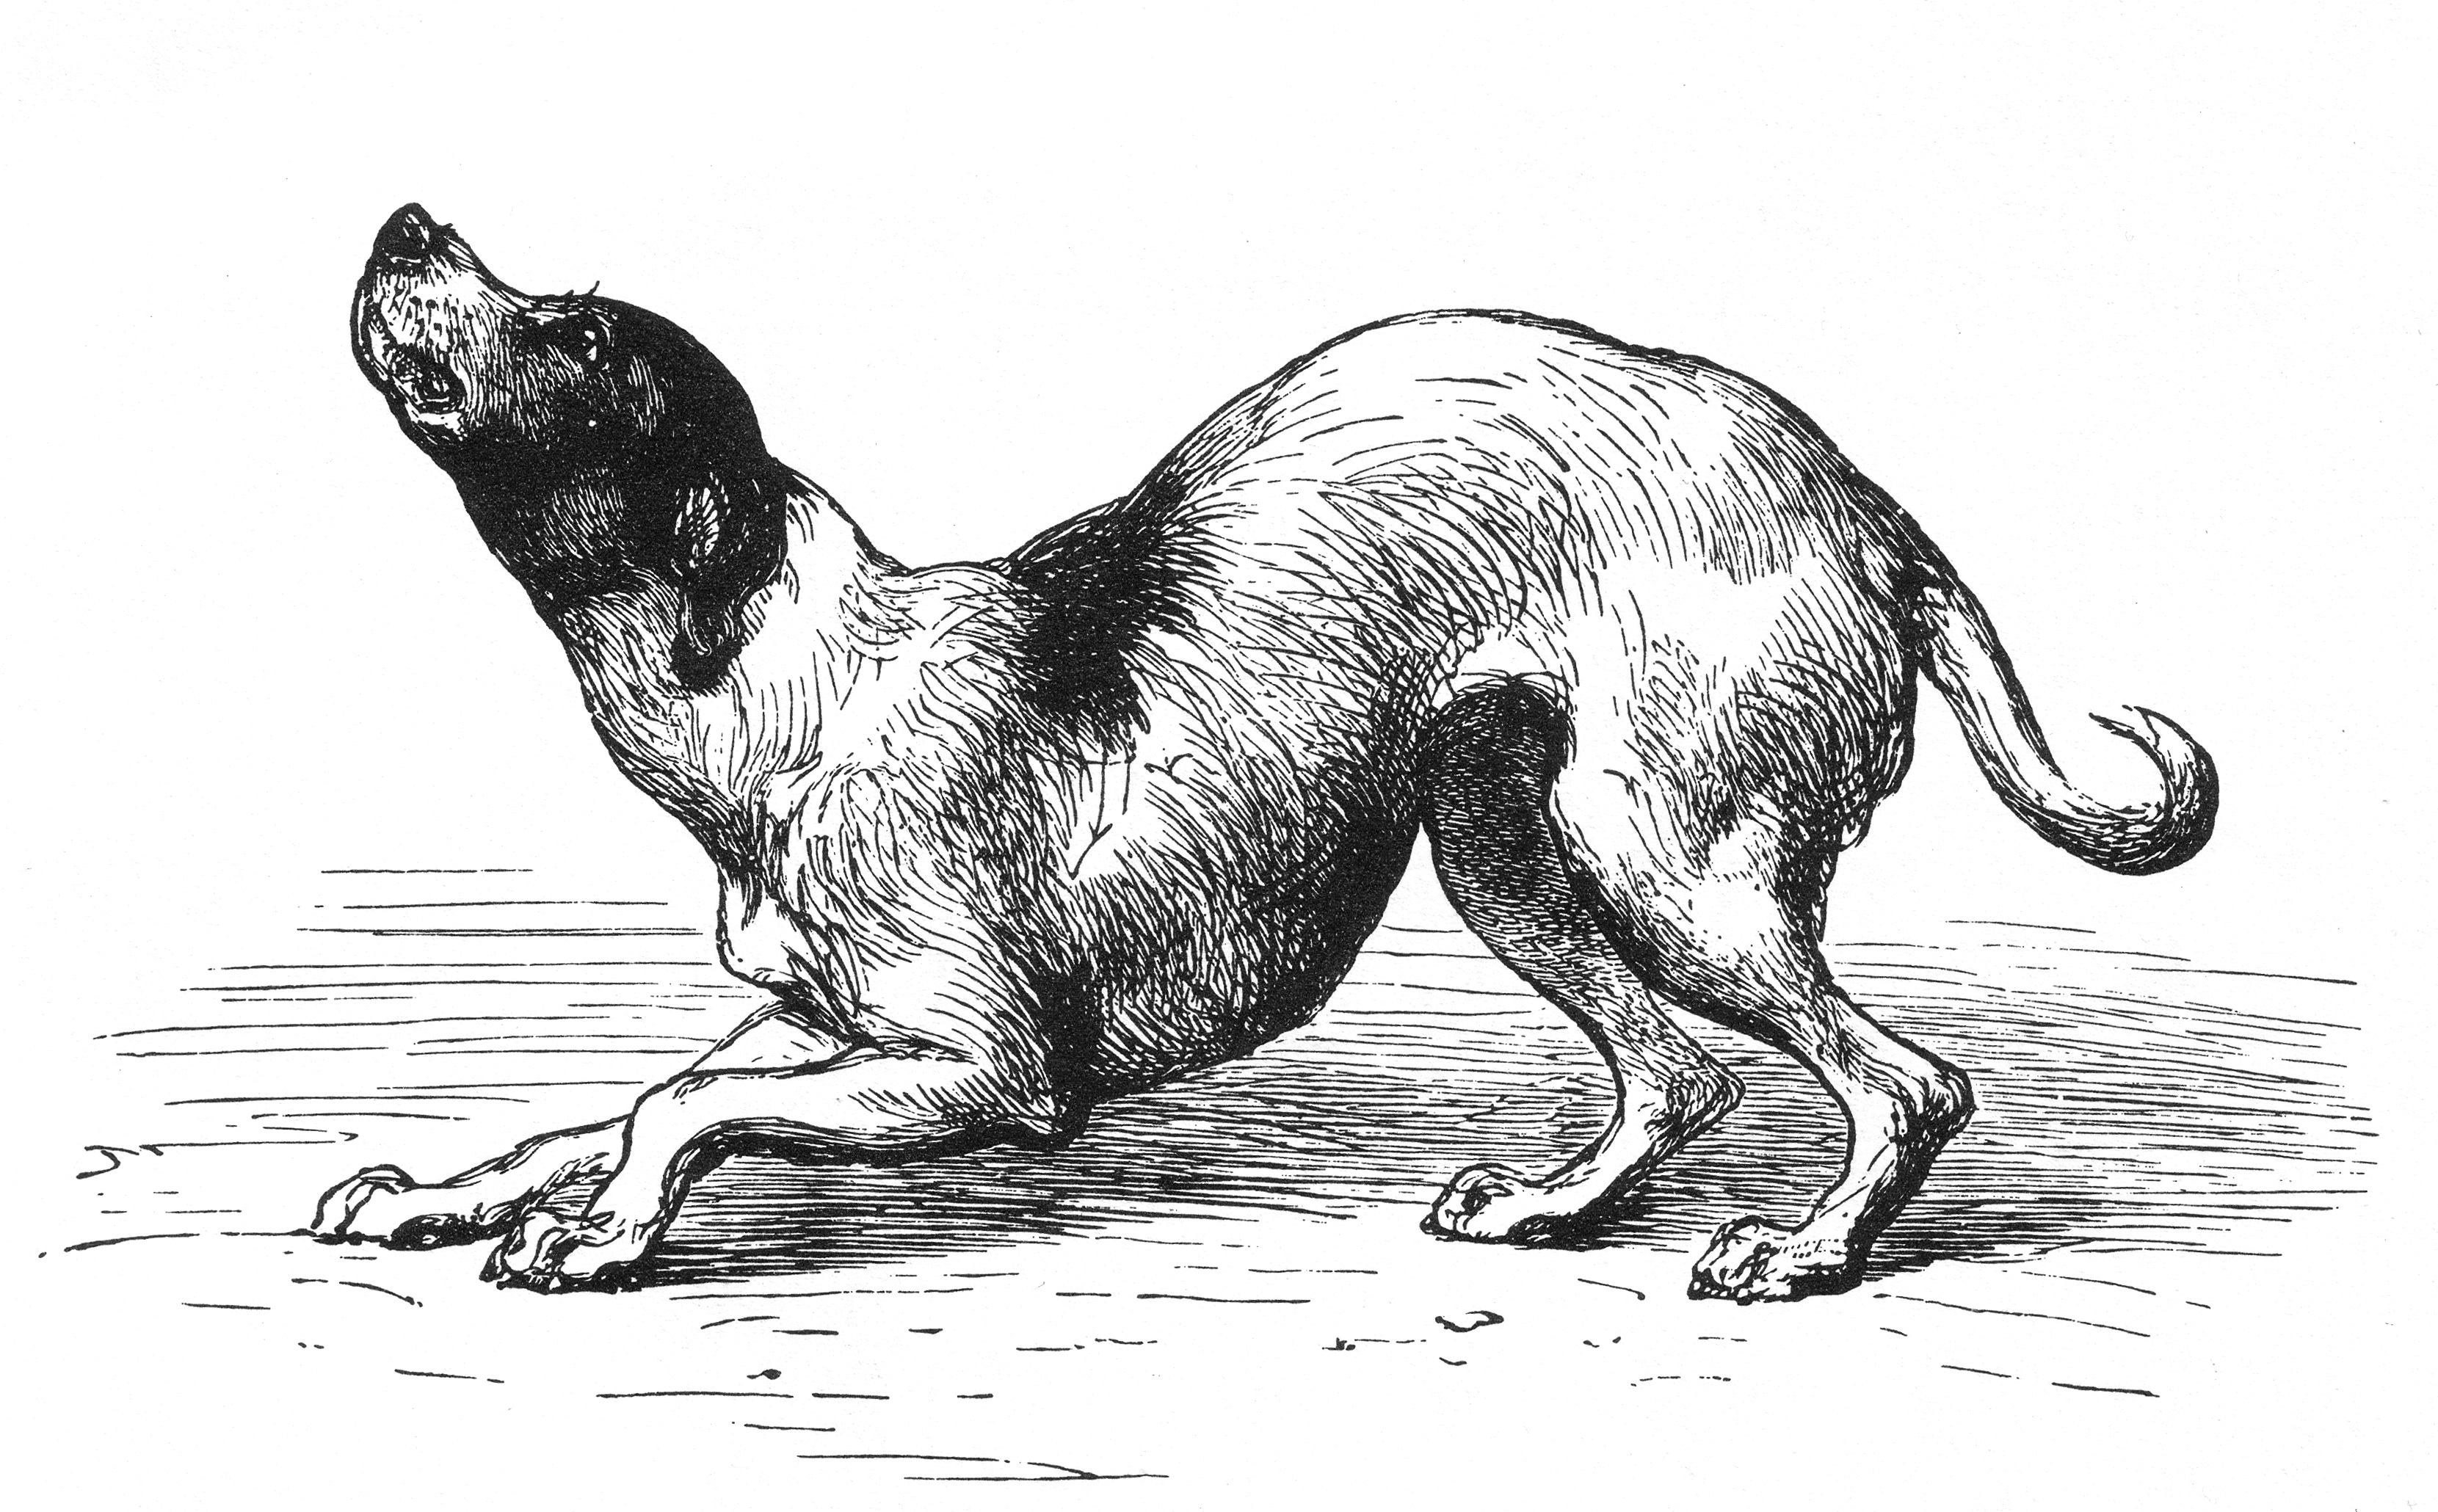
\includegraphics[width=0.70\textwidth,keepaspectratio]{figures/Fig03}
\caption{Darwin's illustration of a dog in an affectionate attitude 
(Figure 6 from \textit{The Expression of the Emotions in Man and 
Animals}).}
\label{darwin2}
\end{figure}




\begin{quotation}
None of $[$these$]$ movements, so clearly expressive of 
affection, is of the least direct service to the animal. They are 
explicable, as far as I can see, solely from being in complete 
opposition to the attitude and movements which are assumed when a dog 
intends to fight, and which consequently are expressive of anger. 
\citep[15--16]{darwin_expression_1872} 
\end{quotation}


\begin{figure}[h]
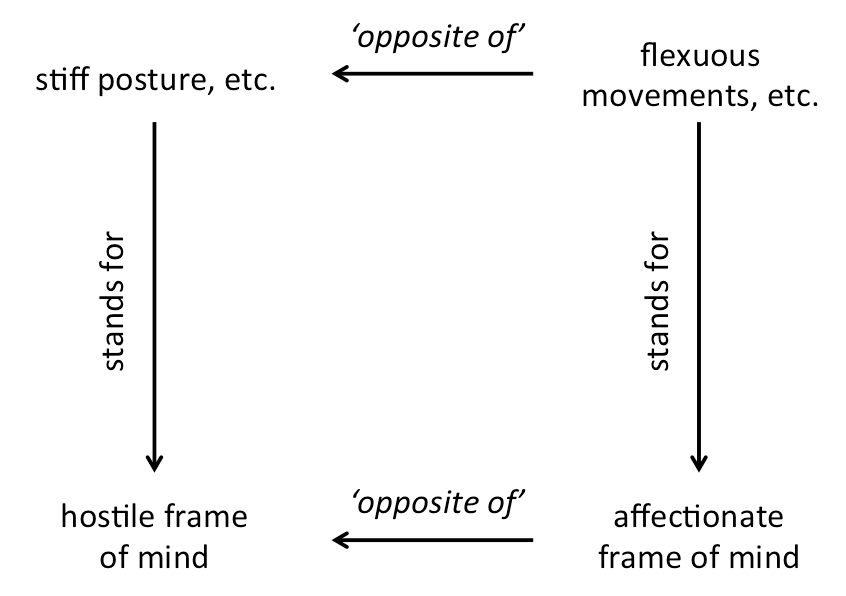
\includegraphics[width=0.55\textwidth,keepaspectratio]{figures/Fig04}
\caption{A secondary indexical association between observable behavior 
and frame of mind (at right), deriving its meaning only in connection 
with the established relation illustrated in \figref{functionalassoc} (and incorporated 
at left of this Figure), assuming the interpreter's knowledge of a 
limited range of possible bodily behaviors, on the one hand, and a 
limited set of frames of mind, on the other (after Darwin).}
\label{secondaryassoc}
\end{figure}

As depicted in \figref{secondaryassoc}, antithesis is a secondary relation. It is a relation between relations. As Darwin 
pointed out, this secondary relation is only possible if the interpreter has already recognized a primary functional relation. But there is something 
more that it depends on, something crucial to the idea of a semiotic 
system. It follows from the meaning of the term \textit{opposite}. 



To see that a certain behavior is `the opposite' of some 
other behavior, as opposed to simply \textit{not} that other behavior, 
you must be able to consider alternative possibilities within a 
restricted set. Flexuous movements can be recognized as the opposite of 
the aggression-signaling behavior only when one knows, or can predict, a 
limited range of postures that a dog can make. For this to work in 
the way depicted in \figref{secondaryassoc}, you must also understand that there is a 
limited set of relevant frames of mind that the dog may have, with aggressive at one end and affectionate at the other. 



This type of semiotic system arises when Darwin's principle of 
antithesis sets up \textit{relations between relations} \citep[12--17]{kockelman_agent_2013}. This becomes possible when someone has access not just to what they are currently perceiving (e.g., a dog in a certain posture) but when the person also knows about other systems such as body 
posture and emotional state, with some sense of their elements 
and the logical-causal relations between them. A person should understand that if a dog is 
being affectionate it is necessarily not being aggressive, or that if 
its body is stiff it cannot also be flexuous. 



Central to the idea of a \textit{functional relation to context} that I am outlining here are the concepts of \textit{incorporation }and 
\textit{contextualization}. These are defined in semiotic terms by 
\citet[29]{kockelman_residence_2006}, as follows:



\begin{enumerate}
\item[]\textit{Incorporation.}\is{incorporation} For any two semiotic processes, A and B, A will be said to incorporate B 
(and hence be an interpretant of it) if the sign of B relates to the 
sign of A as part-to-whole, and the object of B relates to the object of 
A as means-to-ends. For example, in the case of instruments (semiotic 
processes whose sign is an artificed entity and whose object is a 
function), a wheel incorporates a spoke.



\item[]\textit{Contextualization.}\is{contextualization} For any two semiotic processes, A and B, A will be said to contextualize 
B, if A is required to interpret B, or at least assists in interpreting 
B. For example, a hammer contextualizes a nail. And a sword 
contextualizes a sheath. That is, nails make no sense without the 
existence of hammers; and sheaths make no sense without the existence of 
swords.
\end{enumerate}



The concepts of incorporation and contextualization help us to define functional relations. They hold, for example, for the relations 
between a verb and a clause, a handle and a knife, a marriage rule and a 
kinship system.\is{kinship systems} They account for relations between concepts and the larger frames that contextualize them \citep{FillmoreFrameSemantics1982}. They are the basis of combinatoric rules, and as such 
they ultimately account for grammar in the complete sense (assuming a 
semantically-based approach to grammar; cf. \citealt{langacker_foundations_1987,wierzbicka_semantics_1988,croft_explaining_2000,haspelmath_pre-established_2007}). 

%\textit{Note synchronic relations}, but realized/evidenced in microgenetic and enchronic frames; cf. also ontogenetic vs phylogenetic ritualization.

\section{More complex systems}


The basic relations-between-relations structure shown in \figref{secondaryassoc} combines with incorporation and contextualization -- kinds of embedding relations -- to yield the sorts of semiotic systems that make up any natural language 
(\citealt{saussure_cours_1916}; see \citealt{dixon_basic_2010,dixon_basics_2014}, \citealt{bickel_linguistic_2014}). 



All languages have systems of form classes.\is{form classes} The thousands of 
words (and other morphemes) that you have to learn in order to 
speak a language can be categorized according to how they are
distributed relative to each other. There are open classes of 
content words like nouns and verbs (in most if not all languages) versus closed classes of function 
words like prepositions\is{prepositions} (e.g., in English)\is{English} and case-marking\is{case-marking} affixes 
(e.g., in Finnish).\is{Finnish} 



Then there are constructional systems defined by principles of combination. An example is the system for describing motion 
events\is{motion events} in Lao\is{Lao} \citep[387--389]{enfield_grammar_2007}. There are three consecutive 
slots. Each slot may be filled with a 
verb from three distinct sets. The first verb refers to the manner of 
motion (this is an open set). The second refers to the path of motion 
(from a set of 10 verbs). The third refers to the 
direction of motion in relation to the deictic center (from a set 
of 3 verbs). See Table \ref{laodirectionalverbsystem}.


\begin{table}[htbp]
 % \centering
      \begin{tabular}{lll}
  \lsptoprule
    Slot 1 & Slot 2 & Slot 3 \\
    Verb of manner & Verb of path & Verb of direction \\
    (open class) & (closed, n=10) & (closed, n=3) \\
\midrule
    \textit{lèèn1} ‘run’ & \textit{khùn5} ‘ascend’ & \textit{paj3} ‘go’ \\
    \textit{ñaang1} ‘walk’ & \textit{long2} ‘descend’ & \textit{mùa2} ‘return’ \\
    \textit{king4} ‘roll’ & \textit{khaw5} ‘enter’ & \textit{maa2} ‘come’ \\
    \textit{lùan1} ‘slide’ & \textit{qòòk5} ‘exit’ &  \\
    \textit{tên4} ‘jump’ & \textit{khaam5} ‘cross.over’ &  \\
    \textit{lòòj2} ‘float’ & \textit{lòòt4} ‘cross.under’ &  \\
    \textit{khii1} ‘ride’ & \textit{taam3} ‘follow’ &  \\
    \textit{khaan2} ‘crawl’ & \textit{phaan1} ‘pass’ &  \\
    \textit{taj1} ‘creep’ & \textit{liap4} ‘go along edge’ &  \\
    \textit{com1} ‘sink’ & \textit{qòòm4} ‘go around’ &  \\
    \textit{doot5} ‘leap’ &       &  \\
    etc.  &       &  \\
   \lspbottomrule
    \end{tabular}%
    
\caption{Lao directional verb system}  
\label{laodirectionalverbsystem}%
\end{table}%




Using this system, a Lao speaker can say things like this:


\ea
\gll khaan2 qòòk5 paj3 \\
     crawl  exit  go \\
\glt `(S/he/it) crawled out/away.'
\z

\ea
\gll doot5 long2 maa2 \\
     leap descend come \\
\glt `(S/he/it) leapt down here.'
\z

\ea
\gll lòòj2 phaan1 mùa2 \\
     float pass return \\
\glt `(S/he/it) floated back past.'
\z


This linguistic sub-system illustrates a fundamental 
intersection between two axes. A \textit{syntagmatic axis}\is{syntagmatic axis} is the `left-to-right' axis along 
which separate elements combine. On a \textit{paradigmatic axis},\is{paradigmatic axis} each slot along the syntagmatic axis
may be filled by alternative members of a set, with contrast 
effects between possible values (not unlike the way a dog's stiff posture 
is opposed to a flexuous posture). 



Sub-systems in language interact with each other and show dependencies\is{dependencies in systems} 
in higher-level systems like those defined in comprehensive 
grammatical descriptions. \citet{aikhenvald_dependencies_1998} describe 
dependencies among grammatical sub-systems. They point out, for example, that 
the system of polarity\is{polarity} (positive versus negative in relation to a 
predicate or clause) puts constraints on other sub-systems in the grammars of 
many languages. For example, in Estonian,\is{Estonian} there is a system in which person and number are 
distinguished by morphological marking on the verbs, but these 
distinctions are only realized in positive polarity. The distinctions 
are lost in the negative. See Table \ref{verbtobeinestonian}.





\begin{table}[h]
\centering
\begin{tabular}{ll}
\lsptoprule
\textsc{positive} & \textsc{negative} \\
\midrule
\textit{olen} (\textsc{1sg)}, \textit{oleme} (\textsc{1pl}) 
& \\

\textit{oled} (\textsc{2sg)}, \textit{olete }(\textsc{2pl)} & 
\textit{ei ole} (1/2/3\textsc{sg/pl}) \\

\textit{on} (\textsc{3sg/pl}) & \\
\lspbottomrule
\end{tabular}
\caption{Verb `to be' in Estonian}
\label{verbtobeinestonian}
\end{table}


\citet{aikhenvald_dependencies_1998} present a cross-linguistic hierarchy of dependencies between sub-systems like these. This kind of inter-connectedness between 
paradigm sets and combinatoric rules, and between sub-systems in a 
language, is evidence for the broad underlying system properties of 
linguistic behavior. 



It follows from these facts about linguistic systems that we cannot 
view any piece of language as a mere item. ``A living language is not 
just a collection of autonomous parts'', say \citet[1]{donegan_rhythm_1983}. A language is ``a harmonious and self-contained whole, massively 
resistant to change from without, which evolves according to an 
enigmatic, but unmistakably real, inner plan'' \citep[1]{donegan_rhythm_1983}. 



They illustrate their point in explaining how it is that the languages 
of two sides of the Austroasiatic language family\is{Austroasiatic language family} -- Munda\is{Munda languages} and 
Mon-Khmer\is{Mon-Khmer languages} -- show a list of typological distinctions that are ``exactly 
opposite at every level of structure'' \citep[111]{donegan_south-east_2002} 
even though they are known to be descended from the same proto-language. Donegan and Stampe argue that speakers of Munda innovated a new prosodic profile, and when they did this they 
were tampering with something that ``pervades every level of language 
structure'' \citep[14]{donegan_rhythm_1983}. A simple change from iambic to trochaic\is{iambic versus trochaic} stress in words had systemic knock-on effects that changed the entire morphosyntactic profile of the language. Table \ref{mundamonkhmer}
is adapted from \citet[1--2]{donegan_rhythm_1983}.\footnote{Donegan and Stampe of course considered the possibility that language contact\is{language contact} explains the data in Table \ref{mundamonkhmer}. Their goal was to argue against a contact account, with their knock-on effect idea being offered as an alternative. Whether they are right remains an open question. Neither contact nor internal development\is{internal change} can be treated as a null hypothesis. Pronponents of both arguments are obliged to make their case.}


\begin{table}[h]
\begin{tabularx}{\textwidth}{>{\itshape}XXX}
\lsptoprule
 & \textbf{Munda} & \textbf{Mon-Khmer} \\
\midrule
Phrase accent & Falling (initial)                & Rising (final) \\[.3em]
Word order    & Variable-SOV, 
                \mbox{AN, Postpositional}        & Rigid-SVO, 
               \mbox{NA, Prepositional} \\[.3em]
Syntax        & Case, verb agreement             & Analytic \\[.3em]
Word canon    & Trochaic, dactylic               & Iambic, monosyllabic \\[.3em]
Morphology    & \mbox{Agglutinative, suffixing,} 
                 polysynthetic                   & \mbox{Fusional, prefixing} 
\mbox{or isolating} \\[.3em]
Timing        & Isosyllabic, isomoric           & Isoaccentual \\[.3em]
Syllable canon& (C)V(C)                         & \mbox{Unaccented (C)V,} 
       \mbox{accented (C)(C)V(G)(C)} \\[.3em]
Consonantism  & Stable, 
               \mbox{geminate clusters}         & \mbox{Shifting, tonogenetic,} 
       \mbox{non-geminate clusters} \\[.3em]
Tone/register & Level tone (Korku only)         & Contour tone/register \\[.3em]
Vocalism      & \mbox{Stable, monophthongal,}
       \mbox{harmonic}                & \mbox{Shifting, diphthongal,} 
\mbox{reductive} \\[.3em]
\lspbottomrule
\end{tabularx}
\caption{Properties of Munda and Mon-Khmer languages}
\label{mundamonkhmer}
\end{table} 



As the examples discussed here show, there are good reasons to believe 
that languages have higher-level system properties. Yet there is no 
single causal event in which a language as a whole system is transmitted, at least not in the same sense as the single causal event of sexual reproduction by which a full set 
of genetic\is{genetics} information is transmitted in vertebrates.\is{vertebrates} Below, I return to the 
transmission problem. But first, I want to broaden the scope and show that 
the point I have just made for language also holds for social and 
cultural systems. 


\newpage
As an illustration of the system concept in another domain of culture, consider \textit{sections}\is{sections} 
and \textit{subsections}\is{subsections} in Aboriginal Australia\is{Aboriginal Australia} \citep{radcliffe-brown_social_1931}. In a 
section system, all members of a community belong in one of four 
categories. Each category has a name in the local language (e.g., in the 
Alyawarre language of Central Australia\is{Alyawarre} they are \textit{Kngwarriya}, 
\textit{Upurla}, \textit{Pitjarra} and \textit{Kimarra}). For convenience we can label them A, B, C, and D. 



As \citet[2]{mcconvell_origin_1985} describes it, in a four-term section system ``a man 
of A marries preferentially a woman of B; their children are D. A man of 
B marries a woman of A; their children are C. C and D similarly marry 
each other, and their children are A if the mother is C and B if the 
mother is D''. After two generations of this, one ends up in the same 
section as one's father's father or mother's mother. See \figref{sections}.

\begin{figure}[h]
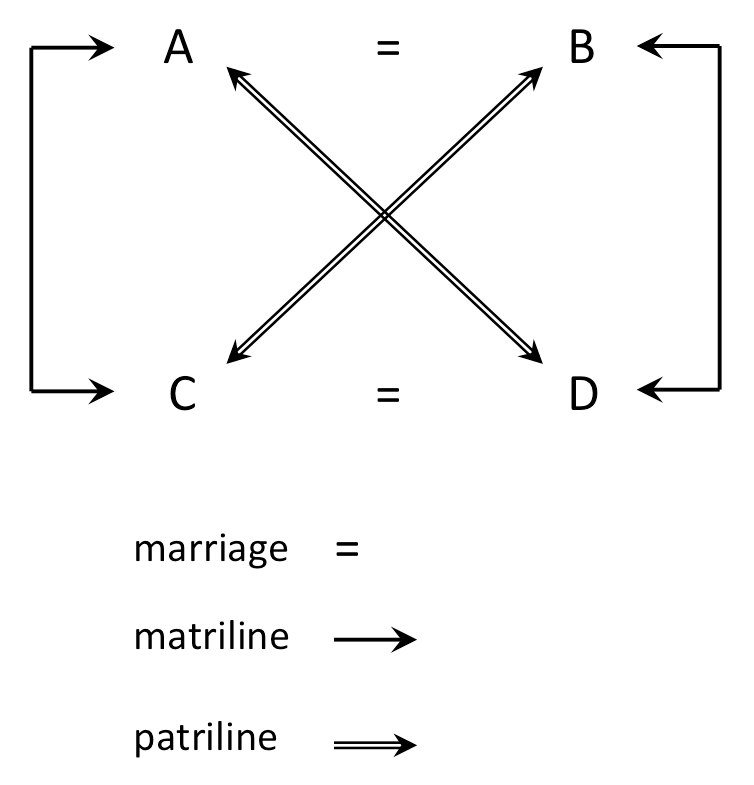
\includegraphics[width=0.5\textwidth,keepaspectratio]{figures/Fig05}
\caption{Sections (Northern Australia), from \citet[32]{mcconvell_origin_1985}, after 
\citet{radcliffe-brown_social_1931}. }
\label{sections}
\end{figure}







McConvell also describes the doubly complex subsection systems. In a subsection system, the four categories of what used to be a section system are each divided in 
two (see McConvell for diagram and discussion). There are structural 
consequences. For example, a cross-cousin is a possible wife in a 
section system, but not in a subsection system. 



These kinds of system are widespread in Aboriginal Australia. They are shared by 
groups that have completely different languages. \citet{evans_enigma_2012} compares the 
situation to that of the modern system of military ranks as officially 
standardized by the Geneva Convention:\is{Geneva Convention} groups in the same culture area have direct translations for the same offices in what is essentially the same system. In Northern Australia,\is{Northern Australia} a common cultural context has 
facilitated the widespread and stable status of particular types of 
kinship systems and vocabularies.\is{kinship systems} 



But there are many aspects of culture that seem less 
like systems and more like items. \citet{eckert_variation_2008} gives the example of a cut of 
jeans that happens to be fashionable\is{fashion} among high school kids one year, though she urges us not to be tempted by the apparent individuability of 
such cultural elements. Something like the wearing of pegged pants or a 
way of pronouncing a vowel is always situated in an \textit{indexical 
field}, as she puts it. When things like these are borrowed or adopted into new 
social settings they may be \textit{segmented} out from a historical and 
indexical constellation of signs and meanings. 



People who do this segmenting may be unaware of the larger (especially 
historical) connections. They will nevertheless give the item a 
place in a new system. \citet{parry_money_1989} make this point in connection with the historical adoption of money\is{money} around the world: ``in 
order to understand the way in which money is viewed it is vitally 
important to understand the cultural matrix into which it is 
incorporated'' \citep[1]{parry_money_1989}.



\citet{sahlins_what_1999} says that when new elements -- everything from 
money to snowmobiles\is{snowmobiles} -- are incorporated into cultural contexts, they are 
adopted for local purposes and given a ``structural position'' in ``the 
cultural totality''. Sahlins celebrates the appropriation 
by neotraditional people of elements from other people 
(and note we can distinguish between processes of appropriation that 
alter the item so as to make it fit into the receiving system versus 
those that alter the system so as to fit the incoming item; usually it is a combination of the two). 



Sahlins is criticizing the idea that cultures like the Yupik\is{Yupik culture} 
become contaminated when people borrow modern innovations. His point is that once the items in question are borrowed, they are changed. They have new meanings in their new contexts. 



\section{Are cultural totalities illusory?}

\is{cultural totalities}
Consider the kinds of systems and relations of incorporation\is{incorporation} in language and 
culture just discussed. They show that we are never dealing with 
detached cultural items. But it does not follow from the striking 
systematicity of Australian sections\is{sections} and subsections\is{subsections} that 
these ramp up into cultural totalities. It's possible that they do. After all, ethnographers have 
succeeded in writing reference descriptions of the knowledge, practices, 
values, and technologies of defined social/cultural groups  \citep{radcliffe-brown_andaman_1922,bronislaw_malinowski_argonauts_1922,firth_we_1936,evans-pritchard_nuer:_1940,fortes_dynamics_1945}. In the same way, linguists have succeeded in describing languages as 
totalities, not in the way a layperson might discretely label an 
imagined language -- Dutch, Flemish,\is{Dutch versus Flemish} Thai, Lao,\is{Thai versus Lao} etc. -- but rather in the technical sense of listing the full vocabulary and set of 
grammatical rules that any speaker in a community should know. 



What is our evidence that such totalities exist? Both the ``whole 
systems'' and the ``parts'' of language seem clearly identifiable at first, but both ideas crumble upon close inspection \citep{le_page_acts_1985,hudson_sociolinguistics_1996}. Any linguist knows that 
``a language'' -- in the sense of a community-wide system like French or 
Korean -- is impossible to define by pointing at 
it: ``as a totality it is inaccessible and indefinable; each of us has 
only partial experience of it'' \citep[191]{le_page_acts_1985}. 



`A language' in the sense that we normally mean it constitutes a system 
insofar as it is a set of interrelated items, such as words, each of 
which appears to be a stand-alone unit or element.\is{languages, as unit of analysis} The system\is{systems} idea is 
especially clear in the case of language for at least three reasons. First, the set of 
interrelated items in a language is a very large set. Second, we have 
strong intuitions about what is part of language and what is not. Third, this set contains numerous \textit{sub-}systems. 
But still we never encounter a language as such, only fragments of 
languages, items like words and grammatical constructions, in contexts of speech and writing. 



In their masterpiece on the nature of language, \citet[8--9]{le_page_acts_1985} challenge us to face the problem of ``how to 
know when to speak of separate systems'': 



\begin{quotation}
If we start from the concept of an underlying system this becomes an 
extremely difficult, if not insoluble, problem; if however we approach 
it from the point of view of the degree of coherence evidenced in the 
behavior of a group of individuals, the problem is seen to be one of 
relationships and of stereotypes inherent in each individual.  
\end{quotation}




Metalinguistic stances\is{metalinguistic stances} are real. But this does not mean that the systems 
those stances point to are real in the same way. How, then, can we have a clear 
causal account of linguistic systems? The answer -- to bring us back to the 
item/system problem -- is in the causality of social behavior at the micro 
level.



%\textit{to insert}: ‘The grammar of the closed system, and its predictions of ‘grammaticality’, become confused with the empirical judgements of people whose concept of ‘grammaticality’ - if they have one at all, which is in fact comparatively rare among the world’s population at large - is subsumed within a much wider concept of ‘acceptability’, a concept which takes account of creative, innovative, analogical, inventive and tolerant capacities of the human mind ignored by the closed systems of many grammarians.’ (Le Page and Tabouret-Keller:194)


